\documentclass[a4paper]{article}
 
\usepackage{amsmath}
\usepackage{graphicx}
\usepackage{caption}
\usepackage{subfigure}
\usepackage{epstopdf}
\usepackage[ansinew]{inputenc}
\usepackage{listings}
\usepackage{xcolor}
%\setlength{\oddsidemargin}{0cm}
%\setlength{\evensidemargin}{0cm}
%\setlength{\topmargin}{0cm}

\usepackage[]{algorithm2e}

\usepackage{a4wide}

\title{ Simulating the mouse brain model constructed from Allen Institute for Brain Science data on the Blue Brain 4 supercomputer }
\author{Till Schumann}
%\date{}

\begin{document}
   \maketitle

\section{Introduction}
\subsection{Brain Simulations}
\subsection{Allen Brain Atlas}
   Allen Institute for Brain Science provides a high-resolution map of neural connections in the mouse brain.
   It contains several injection experiments. The provided datasets of the experiments 
   contain a 3D image of the injection and a 3D image of its axonal projection labeled by viral
   tracers.
   
   \begin{figure}[ht!]
   	\begin{center}
        \subfigure[Injection sites - showing all available experiments]{%
            \label{fig:allInjections}
            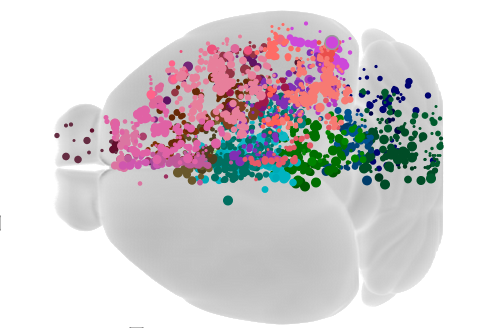
\includegraphics[width=0.4\textwidth]{../connectionBrowser_allinjections.png}
        }
        \hspace{1cm}
        \subfigure[Projection density of one experiment]{%
            \label{fig:oneProjection}
            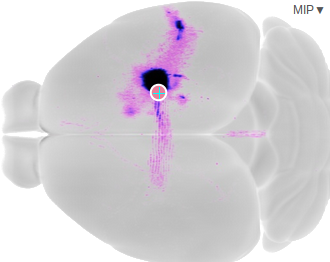
\includegraphics[width=0.32\textwidth]{../connectionBrowser_oneinjections.png}
       }
    	   \end{center}
    	\caption{%
        The pictures are inverted and copied from the Allen Brain Atlas.
     }%
   \label{fig:atlas}
   \end{figure}
   
\subsection{BBP recipe}
	The Blue Brain project   

\subsection{NEST}
NEST is a simulator for spiking neural network models that focuses on the dynamics, size and structure of neural systems rather than on the exact morphology of individual neurons. The development of NEST is coordinated by the NEST Initiative. NEST is ideal for networks of spiking neurons of any size, for example:
Models of information processing e.g. in the visual or auditory cortex of mammals, models of network activity dynamics, e.g. laminar cortical networks or balanced random networks and models of learning and plasticity. A NEST simulation tries to follow the logic of an electrophysiological experiment that takes place inside a computer with the difference, that the neural system to be investigated must be defined by the experimenter. The definition is based on number of neurons with parameters and connections between these neurons. NEST supports the generation based on probabilistic values. The stochastic settings of a neuronal network can be used to create its artificial copy inside of NEST. To manipulate or observe the network dynamics, the experimenter can define so-called devices which represent the various instruments (for measuring and stimulation) found in an experiment. These devices write their data either to memory or to file. 

\subsection{Visualization}
To interpret the output of a neuronal simulation the spiking activity of the neurons is analyzed, mostly. Different types of methods allow to extract stochastic characteristics from spike trains. Besides this visualization of the spike trains taking their location into account, allows to create a video, which shows the activity of the neuronal network.

\section{Methods}
\subsection{Interfaces}
\subsection{Circuit generation}

\subsubsection{Long range connections}
A set of experiments is used to connect neurons located at the injections
to the neurons at the projections. Unfortunately all injections from these experiments do not
cover the whole brain. So there are neurons which are not injected
by any experiment. Therefore all neurons which are not injected should use the projection
from the nearest injection. To map pixels of the 3D pictures to neurons, the neurons are assigned to voxels, which represent the pixels. In a first step the best experiment is chosen for each voxel based on the minimal total injection per experiment. In the second step all voxels in the right hemisphere, which have not received an experiment take the experiment from the nearest voxel, which has an experiment. In the third step the given experiments are used to generate the connections for the related neurons. To get connection for the both hemispheres the information is mirrored along the z-axis.

\begin{figure}[ht!]
   	\begin{center}
        \subfigure[Illustration injection]{%
            \label{fig:allInjections}
            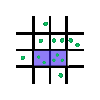
\includegraphics[width=0.15\textwidth]{cg_illustration_injection.eps}
        }
        \hspace{0.5cm}
        \subfigure[Illustration projection]{%
            \label{fig:oneProjection}
            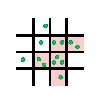
\includegraphics[width=0.15\textwidth]{cg_illustration_projection.eps}
       }
       \hspace{0.5cm}
       \subfigure[Merge experiment]{%
            \label{fig:allInjections}
            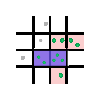
\includegraphics[width=0.15\textwidth]{cg_illustration_merge.eps}
        }
        \hspace{0.5cm}
        \subfigure[specify source and target neurons]{%
            \label{fig:oneProjection}
            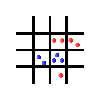
\includegraphics[width=0.15\textwidth]{cg_illustration_neurons.eps}
       }
    \end{center}
    	\caption{%
        Assign density of experiments to neurons.
     }%
   \label{fig:atlas}
   \end{figure}
   
\subsubsection{Short range connections}
The Blue Brain Project has investigated over the last years in experiential work the relation of different synapse types.
They collected their findings in a recipe which allows to get the synapse type for different neuron types.
The neuron types depend on their layer, electrical and morphological type. The recipe defines which synapses are between 
which kind of neurons. The generated synapses connect neurons to its neighborhood. The neighborhood is defined as a
column in the same orientation as the neuron has.

\subsection{Stochastic-driven simulation}
The standard use-case for the NEST simulator is a stochastic-driven simulation. This means
that the circuit is characterized by stochastic parameters (e.g. number of synapses between neurons).
The circuit is build-up inside of NEST using only these parameters.
This means that the amount of need data is small. It allows to build-up large scale simulation
with a few arguments.
\subsection{Data-driven simulation}
As we generated the circuit in a preprocessing step. Neuron and point to point synapse information are given.
Thus we call it a data-driven simulation. We do not use the build-up functionality from NEST.
Hence we have to load the whole circuit from file.

\subsection{Parallel IO}
Build-up a large scale neuronal network from point to point connectivity results in new requirements for data processing and the data format. The parallel IO is strictly limited by the given bandwidth. Clumsy parallel IO access can even lower the resulting bandwidth.
Thus the distribution of the parallel loading has to be carefully chosen. HDF5 allows parallel access to the same file.

\section{Results}
\subsection{Pipeline}
The requirements for all implementations are the usability for the scientists. Besides efficient implementation the users should be able to manipulate the data on different levels. Creating one simulation from data based on the Allen Brain Institute is not the main goal of this thesis. In fact the implementations should complete the tool chain to run data-driven simulations with NEST and visualize them, based on Allen injection experiments. Therefore the proposed pipeline contains data formats which can be manipulated. Processing the needed amount of data takes time and has to be executed on large compute clusters. Thus an interactive usage of the tools is not reasonable.

\subsection{Data format}


\subsection{Circuit generation}
Rewriting the sequential python script to a hybrid C++ application require a parallel implementation of a parallelization strategy and the usage of 
a parallel random generator. For the parallelization strategy a Master-Slave approach is chosen to distribute the workload dynamically on the nodes.
Communication between the individual nodes is not necessary. Only the workload management is handled by the master node.
For the random generator Random123 is used, because good performance and easy usability.
\subsection{NEST Implementation}
\section{Discussion}
\subsection{Parallel Efficiency}
\subsection{Usability for Scientists}

\end{document}
